
\todo[caption={Rozdział inwalida}, inline]{Cały rozdział do przeorania, czy jest już znana interakcja z shutterem, zarys? Wyzwalanie zewnętrzne?}
\subsection{Introduction}
Abcabc

\begin{figure}[H]
\centering
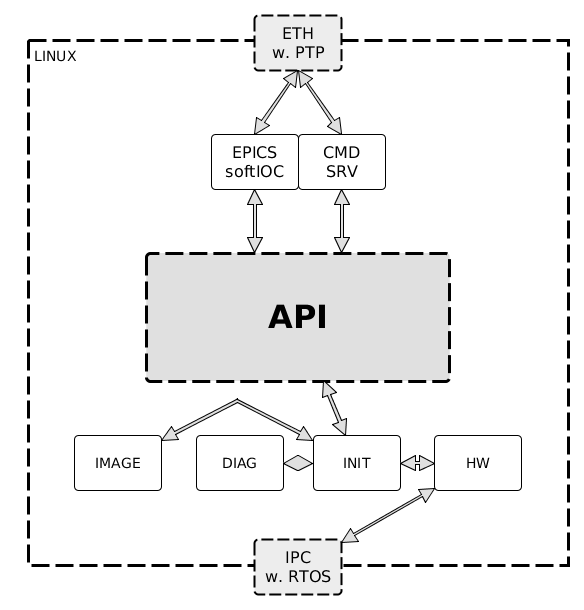
\includegraphics[width=0.6\textwidth]{pict/linux_over.png}
\caption{Neostel camera control}
\label{fig:oses}
\end{figure}

\subsection{RTOS heartbeat}
\todo[inline, caption={heartbeat}]{Tu nie chodzi o heartbeat z RTOSa, tylko heartbeat z Linuksa do zewnętrznego watchdoga; poniższy tekst powinien zostać przeniesiony do rozdziału Diagnostyka \ref{chap:diag} (co już zostało zrobione). Poniższy tekst należy zamienić na opis w jaki sposób będzie z poziomu Linuksa obsługiwany zewnętrzny watchdog /MB}
There won't be any special keepalive nor heartbeat mechanism. The information about presence and proper operation of RTOS will be based on time elapsed since last communication (eg. diagnostic readout). Since Linux OS is master node for all of the IPC transmission there will be RTOS reset mechanism implemented in Linux.

\subsection{Camera control master }
	\todo[inline, caption={Rozdzial o niczym}]{Ten rozdzial jest w tej chwili o niczym, API, ktore jest dostepne z CS bedzie stworzone na podstawie funkcji RTOS/FPGA, wielkiej filozofii nie przewiduje/PZ}
Camera control master is a software entity running on Linux OS providing high level abstraction over RTOS camera control. It acts both as a bridge (using IPC) between Linux OS and RTOS, and provides high level camera control API for Linux user. It abstracts data and command exchange mechanisms.

\subsection{Epics Server}
\todo[inline, caption={EPICS - brakuje inputu od CGS}]{Brakuje inputu odnosnie integracji z otoczeniem, jaka architektura, jakie wymagania? - zalozenie bedzie na poczatek, ze nie implementujemy alarmowania itp. trigerowanego przekroczeniem thresholdow ani przeprowadzania akcji czy uzywania bardziej zaawansowanych funkcjonalnosci niz odczyt parametru i wywolanie jakiegos callbacka z API/PZ}
EPICS soft IOC is used for providing handlers for the API procedures based on an IOC database. 
EPICS enables the facility control software to easily access the functionalities implemented in the camera including:
\begin{itemize}
\item Triggering actions performed by firmware and/or hardware
\item Reading values from the system
\item Implementing alarms and alarm monitoring of values of diagnostic procedures implemented in the camera
\item Periodic scanning of values provided by system components
\end{itemize}
The EPICS server is based on a Channel Access protocol implemented over the TCP/IP protocol and the gigabit Ethernet connection.

\subsection{Monitoring and diagnostic process (DIAG)}

\subsection{API}
\todo[inline, caption={API descr}]{Opisac funkcje API, mocno zalezne od IPC z RTOS}

\subsection{INIT}
\todo[inline, caption={INIT proc desc}]{Opisac proces INIT - nadrzedny, respawnowany automatycznie przez INITa Linuxowego, nadzorca innych procesow systemowych, przeprowadza tez arbitraz dostepu do struktur wspoldzielonych w obrebie linuxa i pilnuje zeby wszystko dzialalo}

\subsection{IMAGE}
\todo[inline, caption={IMAGE proc descr}]{Opisac proces przeprowadzajacy przetwarzanie danych obrazowych (takze tworzacy FITS)}

\subsection{HW}
\todo[inline, caption={HW proc descr}]{Opisac proces zapewniajacy funkcje obslugi HARDWARE i abstrakcje do IPC - po przelozeniu juz na funkcje obslugujace HW}

\subsection{PTP}
\todo[inline, caption={opis PTP}]{Opis PTP wg dokumentacji dzialania uslug ptp4l z phc i hw timestampem na podstawie zrodel z netu, ewentualnie wlasne rozwiazanie bazujace na przerobieniu sterownika sieciowego i dodanie do emacps xilinxowego automatycznego pollingu czy pakiet jest typu PTP i wciagniecie przeliczania czasu do rejestrow, teraz jest to robione w linuxptp \(ptp4l\), jest kilka opcji, mozna poczekac, moze xilinx sam rozwiaze problem/PZi}

%to będzie opisane w sekcji Linux-RTOS IPC
%\subsection{IPC implementation}
%\todo[inline, caption={implementacja IPC w Linuxie}]{Dopisac implementacje IPC w linuxie - podstawowe pytanie czy bedzie to prosta implementacja w userspace, czy tez moze jakis modul kernela napisany na bazie jakiegos frameworka}

\subsection{Cross compile toolchain}
\todo[inline, caption={opis toolchaina}]{opis toolchaina uzywanego do cross compile, skad brany, wersja}

\subsection{Yocto/BSP}
\todo[inline, caption={Opis budowania rootfs}]{Opis budowania rootfs - z mozliwoscia migracji np. na mentora, ktory tez ma komercyjna wersje Yocto albo na Windrivera. Do tego opis BSP, na ktorym bazujemy}

\subsection{Linux Kernel}
\todo[inline, caption={Opis kernela linuxa}]{Opis kernela linuxa - podstawowe parametry configu, co i jak zostalo spatchowane, wersja kernela, do tego device tree}

\subsection{Linux libraries etc.}
\todo[inline, caption={linux lib. list}]{Opisac pakiety kompilowane do rootfs i uzywane biblioteki, jesli jest cos z licencja, ktora moze nakazywac publikacje kodu zrodlowego (zarazliwa), czy dynamiczne linkowanie - trzeba to opisac}

\subsection{U-Boot}
\todo[inline, caption={bootloader}]{Opisac szczegoly uzywanego bootloadera, wersja, modyfikacje, skrypt startowy, env. etc.}


\subsection{Deployment}
\todo[inline, caption={deployment}]{Opisac sposob wdrazania/wrzucania softu po uzyskaniu zrodel, co, gdzie i jak idzie, co jeszcze trzeba zrobic zanim sie uzyska dzialajace rozwiazanie na sprzecie, wlaczajac soft Xilinxa do generowania boot.bin}

\subsection{Testing}
\todo[inline, caption={Brakuje procedur weryfikujacych poprawnosc dzialania}]{Nalezaloby ulozyc scenariusz do testow rozwiazania uwzgledniajacy: funkcjonalnosc, stabilnosc, sprawdzenie granicznej wytrzymalosci, sprawdzenie poprawnosci wypluwanych danych - na tej podstawie mozna potem dobrze diagnostyke napisac. Dodatkowo przydaloby sie dopisac kawalek odnosnie unit testow i sposobu pisania kodu - rowniez w kontekscie wymagan ESA/CGS. Dobrze by bylo opisac narzedzia i wersje zrodel/kompilatorow. /PZi}

\subsection{Optim, debug and profiling}
\todo[inline, caption={tools and techniques for sw. refactoring }]{Opisac narzedzia uzywane do debugowania kernela m.in. LTTNG, softu, GDP, TCF, profilery i inne przydatne narzedzia do analizy zarowno kodu jak i jego wykonania}